% Chapter 2

% variables
\newcommand{\pdirtwo}{chapters/plots/chapter2}

\chapter{The NA64 experiment}

\label{chapter2}

% ----------------------------------------------------------------------------------------

In this chapter, we will describe the NA64 setup in detail. In Sec.\ref{ch2:sec:experimental-technique}, we will clarify what are the main requirements for each of the two decay channels that are being probed by the NA64 experiment. The experimental method is outlined together with the possible challenges to be solved. The two setups share many similarities, and indeed it is quite straight-forward to modify one into the other by changing the detectors configuration. In the case of the invisible mode, a single calorimeter is used as an active target to trigger the $\DM$ production, which is assessed by missing energy in the final state. In the visible mode, a second calorimeter is placed downstream the main target, and the production of $\DM$ is detected by matching the energy of the $\ee$ in the $\aee$ decay with the one deposited by the initial em-shower inside the active dump. In both cases, a well-defined initial state is required, together with a longitudinal hermeticity to avoid any energy leak. In Sec.\ref{ch2:sec:experimental-setup} an accurate description of both setups is given, and we will describe how the challenges outlined in Sec.\ref{ch2:sec:experimental-technique} can be tackled experimentally. The initial particle momentum is measured using a magnetic spectrometer with high-resolution tracking stations. These trackers were under my responsibility during data taking/analysis. The energy is then reconstructed in an active target segmented both longitudinally and transversely. The energy deposited in each cell is used to characterize the incoming particle ID. For the same purpose, Synchrotron Radiation emitted during the passage through the magnetic field is also measured and used to distinguish electrons from hadrons and muons. The installation/commissioning and responsibility during data taking of the first version of this detector made of BGO crystals was also one of the tasks I was responsible for. The analysis of the data and the comparison of the simulation I performed were published in \cite{Depero:2017mrr}. These measurements have shown the advantage of using the detector granularity to greatly enhance the suppression of hadrons and muons contamination in the electron beam at a level of $10^{-5}$. As will be explained in Sec.\ref{ch3:sec:bkg-srd}, this is an essential tool for background suppression in NA64. An introduction of the different types of trigger configurations is also provided to distinguish between data collected at different conditions.
Finally, a description of every single detector is given in Sec.\ref{ch2:sec:detectors}, to highlight the technical details of the different elements used during data taking. 

\section{Experimental Technique}
\label{ch2:sec:experimental-technique}

The detection of the $\DM$ needs to follow different strategies depending on the dominant branching ratio. If $\DM$ decays mainly into $\dmchi$, we saw in chapter \ref{chapter2} that the two possibilities are a beam-dump experiment, where the $\chi$ is detected in a far away detector shielded by a thick wall, or the missing energy technique, where the signature is the missing energy after $\DM$ production. This last technique is the one used by NA64 for its search for Dark Matter. As introduced in chapter \ref{chapter1}, it has the advantage of producing $\DM$ with a rate $\sim \epsilon^2$ instead of the scaling $\sim \alpha_D \epsilon^4$ expected for beam-dump experiments. The key aspects of this experiment are the following:

\begin{itemize}
\item The initial momentum of the particle needs to be known.
\item The setup needs to be completely hermetic, i.e. no energy can escape detection at the level of the experimental sensitivity using channels predicted by the Standard Model.
\item The initial particle ID needs to be known.
\end{itemize}

While the two first items are self-evident since we are looking for missing energy, one could wonder why the last one is necessary. The particle ID is essential to reject background events mimicking the $\DM$ signature. One example is the decay chain $K^- \to e^- \nu_e$ \cite{review-particle-physics}: if a $K^-$ decays in front of the target, the electron will leave an electromagnetic signature in the ECAL and at the same time some energy will be transported out of the setup via the $\nu_e$. This is exactly the signature we would expect for $\DM$ in the invisible mode! Hence the necessity of some system able to distinguish electrons from other particles. Also,  to apply the statistical analysis of the data, one has to know the total number of the electrons that impact our target, the so-called Electrons On Target (EOT). Because of the low contamination in the H4 beam, this impurity is not larger than $\sim1\%$.

What about the visible mode? If we assume the decay $\aee$ is dominant, missing energy can no longer be a signature. One should instead search for a $\ee$ pair in the final state, but these particles are very common in particle physics experiments due to pair-production in the em-shower. The challenge is to select only pairs coming from a Dark Matter decay. Due to its small coupling with ordinary matter, a Dark Photon will travel inside very dense materials with no interaction. Therefore if a high-energetic $\ee$ pair with an energy matching exactly the one missing from the target is measured, one can conclude that the energy was transported outside the volume by a neutral particle. Assuming that we are able to reject all channels in the SM capable of doing the same, we can claim the observation of an event compatible with our hypothesis. Notice that also in this case the three properties listed above are necessary, however, the signal is not missing energy, but instead, energy conservation between the target and a second detector placed downstream (see \ref{fig:two-signature}).
The difference between the two signatures can be addressed in a 2D plane. For the invisible mode, events are binned in the plane $(E_{ECAL};E_{HCAL})$, and the signal region is defined as missing energy in the target and no activity in the Hadronic calorimeter. For the visible mode, the signal requires the initial beam energy to be conserved between the target and a second calorimeter placed downstream to it, with a significant amount of energy leaking from the dump.

Although it is easy to demonstrate that these two signatures are clean using toy simulations, to probe the $\umodel$ one has to collect at least $>10^{10}$ EOT. When such a large statistic is collected, background can arise from very unlikely interactions that are not straightforward to compute. The setup should not only fulfill the key aspects described above but also allow one to suppress as much as possible all the background sources that could leak in the signal box.

\begin{figure}[bth!]
  \centering
  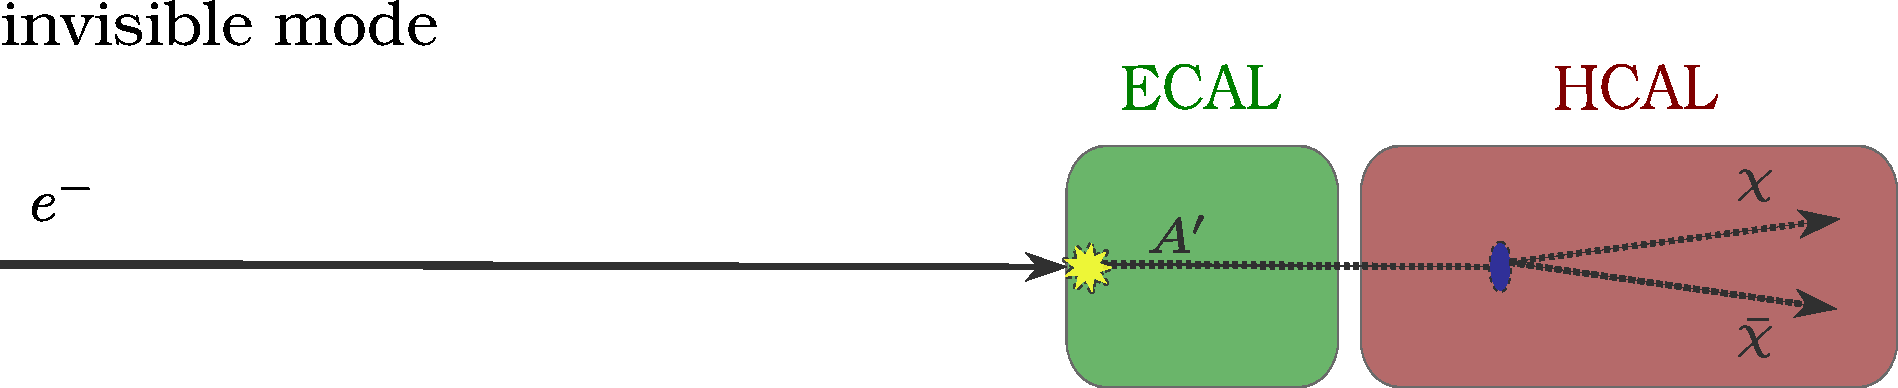
\includegraphics[width=\textwidth]{\pdirtwo/experiments-concepts-invisible.pdf}
  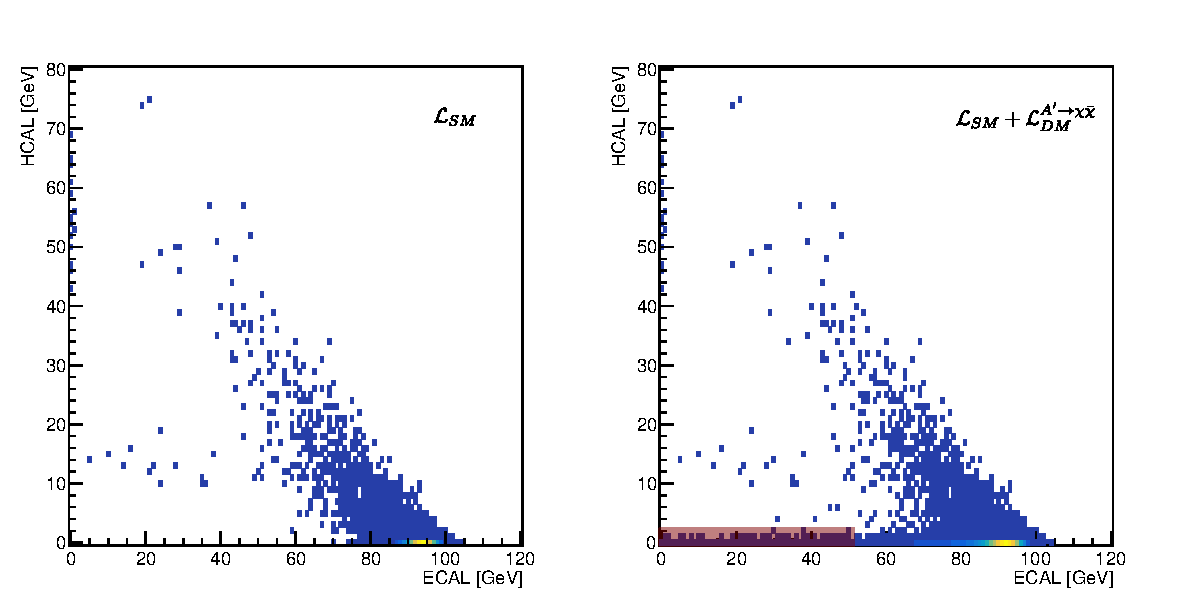
\includegraphics[width=\textwidth]{\pdirtwo/invisiblemode_signalregion.pdf} \\
  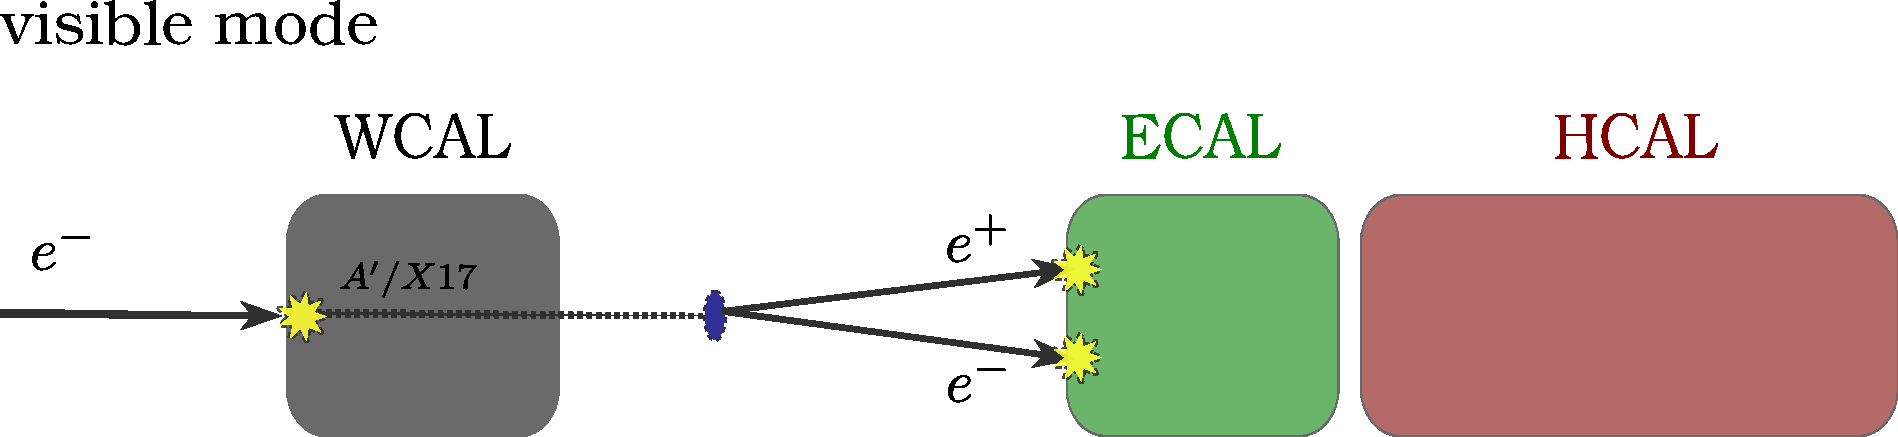
\includegraphics[width=\textwidth]{\pdirtwo/experiments-concepts-visible.pdf}
  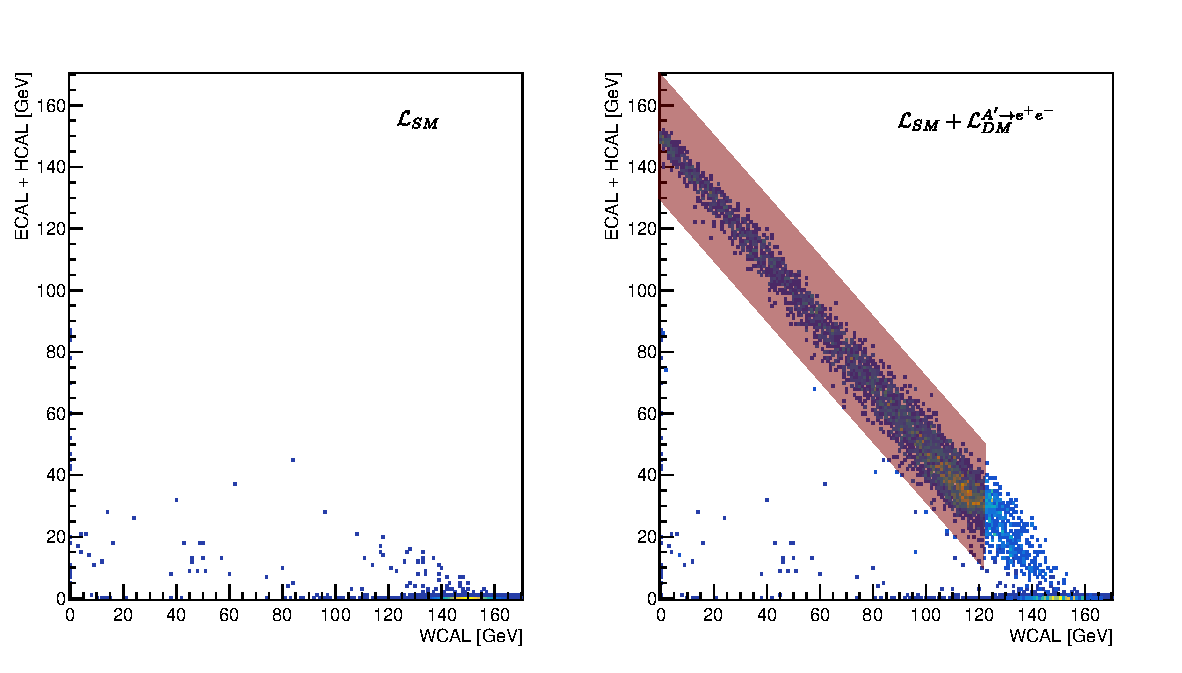
\includegraphics[width=\textwidth]{\pdirtwo/visiblemode_signalregion.pdf}   
\caption[Sketch of experimental signatures for $\DM$]{Sketch of the two possible signatures in the NA64 setup to probe the $\DM$ existence. A heatmap presents the event distribution in the two setups, using only standard model physics (left column) and after adding the Dark Photon production in the simulation (right column). This is done assuming invisible mode decay $\ainv$ (top) or visible mode decay $\aee$ (bottom). In both cases, the signal region of the experiment is drawn as a shaded area.}
\label{fig:two-signature}
\end{figure}

\clearpage
\newpage

\section{Experimental setup}
\label{ch2:sec:experimental-setup}

The NA64 experiment uses the upgraded H4 electron beamline at CERN SPS. The beam is produced by the primary proton beam of 450 \si{\giga\electronvolt} with an intensity up to 5-7$\times$10$^{12}$ Proton On Target (POT) per SPS spill. The electrons are produced on a primary beryllium target and transported to the detector inside the evacuated beamline tuned to an adjustable beam momentum. A precise description of the beam apparatus is available in \cite{sps-beamline,h4-beamline}. The beam properties can be tuned with the magnetic field settings and other parameters. In the case of NA64, two different beam settings are used depending on which $\DM$ decay channel is being probed. In the case of the invisible decay $\ainv$, the beam momentum is tuned to 100 $\gev$. In this condition, a purity $\pi^-/e^- \lesssim 10^{-2}$ is achieved with a beam size of $\sim$\SI{1.5}{cm} (FWHM). In the case of the visible decay $\aee$ on the other hand, larger initial energy is used to boost the decay time of the $\DM$ and increase its chances of traveling outside the target. This is fundamental for the $\DMX$, since an important portion of the parameter space justifying this anomaly is characterized by large couplings $\epsilon \gtrsim 10^{-3}$ and hence a very short decay time $\tau \lesssim 10^{-13}$\si{s}. In this case, the beam is tuned to 150 $\gev$ as a compromise between a high-energy and acceptable reduction of the flux.

In the next sections, both setups used by NA64 will be described in detail. We will follow here a historical approach where the invisible mode setup is described first, as it was originally the first setup used in the test beam of 2015 and the first physics run in 2016. In Sec.\ref{ch2:sec:vismode}, on the other hand, we will focus on the most important difference between this setup and the one used to probe the visible mode.

\subsection{The invisible mode setup}
\label{ch2:sec:invismode}

The invisible mode setup used for data-taking in 2018 is presented in Fig.\ref{fig:setup-invis-2018}. After the e$^-$ primary enters the setup, its momentum is measured precisely with a magnetic spectrometer. It provides an integrated field of $\sim 7$ \si{\tesla\meter} generated by two dipole magnets \cite{mbpl} placed in series along the primary beam-axis. The entrance angle of the particle inside the magnet is defined by two Micromegas (MM) trackers placed inside the 5 m space between the beam inlet and the first magnet entrance. Between the two MM, in a space of approximately 2 m, two scintillators ($Sz_{0-1}$) and a $V$ counter ensure a proper beam definition. The $V$ counter consists of a scintillator with a hole in the middle. Its role is to reject particles with a high beam divergence that could be a potential source of background. The two magnets are followed by a \SI{10.2}{\meter} long vacuum tube kept at 10$^{-3}$ \si{mbar} placed immediately after with a total length of 10.2 \si{m}. The vacuum minimizes the interaction of particles during their travel to the target. This is important to suppress the emission of secondary particles before the primary hits the target. As will be detailed in Sec.\ref{ch3:sec:bkg-srd}, the electron identification achievable with synchrotron radiation is also improved. After the vacuum tube, a space of $\sim$ \SI{4.5}{\meter} contains the last detectors before the target. A second set of three scintillators ($S_{2-3-4}$) completes the trigger system. Three sets of Pb-Sc sandwiches are placed in the arch contained between the original beam and the bent beam direction to collect the synchrotron radiation emitted in the magnetic field upstream. On the other side of the beam (see Fig.\ref{fig:setup-invis-2018}), a similar detector with no transversal segmentation (W in the drawing) rejects events with high beam divergence or events in which the electron experienced a high-energy scattering upstream. Four additional MM (MM$_{3-4-5-6}$) are located along the beam direction to complete the momentum reconstruction by detecting the displacement of the electron after its passage through the magnetic field. Six more tracking detectors are placed before the ECAL: 2 Strawtubes (St), and 4 four Gas Electron Multiplier (GEM). The GEM detectors have a hit resolution and efficiency similar to the MM.
The Strawtubes, on the other hand, have a larger active area (200$\times$200 $\mms$), but a hit resolution of $\sim$1 $\mmi$ which makes them less suitable to reconstruct the momentum precisely \cite{Volkov:2019qhb}. However, due to their large active surface, they can be used to reject rare events where the production by inelastic scattering of hadrons emitted at large angles causes some momentum to escape the setup transversely. These events are not rejected by the W alone and they can be a source of background for the experiment \cite{na64-prd}. 

After this region, the primary electron hits the active target (ECAL). The ECAL is made of 36 modules arranged in a 6$\times$6 matrix, each module has a Pb-Sc structure with 150 layers for a total of 40$X_0$. Due to its transverse segmentation, the ECAL allows further background rejection using a shower profile analysis to distinguish between an em-shower and a hadronic one. To ensure complete hermeticity, a high-efficiency VETO and a large Hadronic Calorimeter (HCAL) are placed after the ECAL target. The VETO consists of three separate scintillators stacked together resulting in a thickness of \SI{5}{\centi\meter}. Its rejection efficiency of Minimum Ionizing Particles (MIP) was estimated to be 99.9$\pm$0.1\% by using muons from calibration runs. The HCAL, located immediately after, consists of four modules of $\simeq$7 $\lambda_{int}$ (nuclear interaction length) each. Each module is built in a 3$\times$3 matrix of a single Fe-Sc sandwich array. The role of the HCAL is to detect the particles (hadrons, neutrals, and muons) penetrating the ECAL to grant energy hermeticity. In the past version of the setup, all four modules were stacked in series after the ECAL for a total of $\simeq$28 $\lambda_{int}$ \cite{Banerjee:2016tad}. In the last version used in 2018, the last module was shifted to face the original beam axis (Fig.\ref{fig:setup-invis-2018}). This allows to detect large Bremsstrahlung photons emitted before the magnet by the incoming electrons. A more detailed description of the NA64 detectors can be found in Sec.\ref{ch2:sec:detectors}.

\begin{figure}[tbh!]
  \centering
  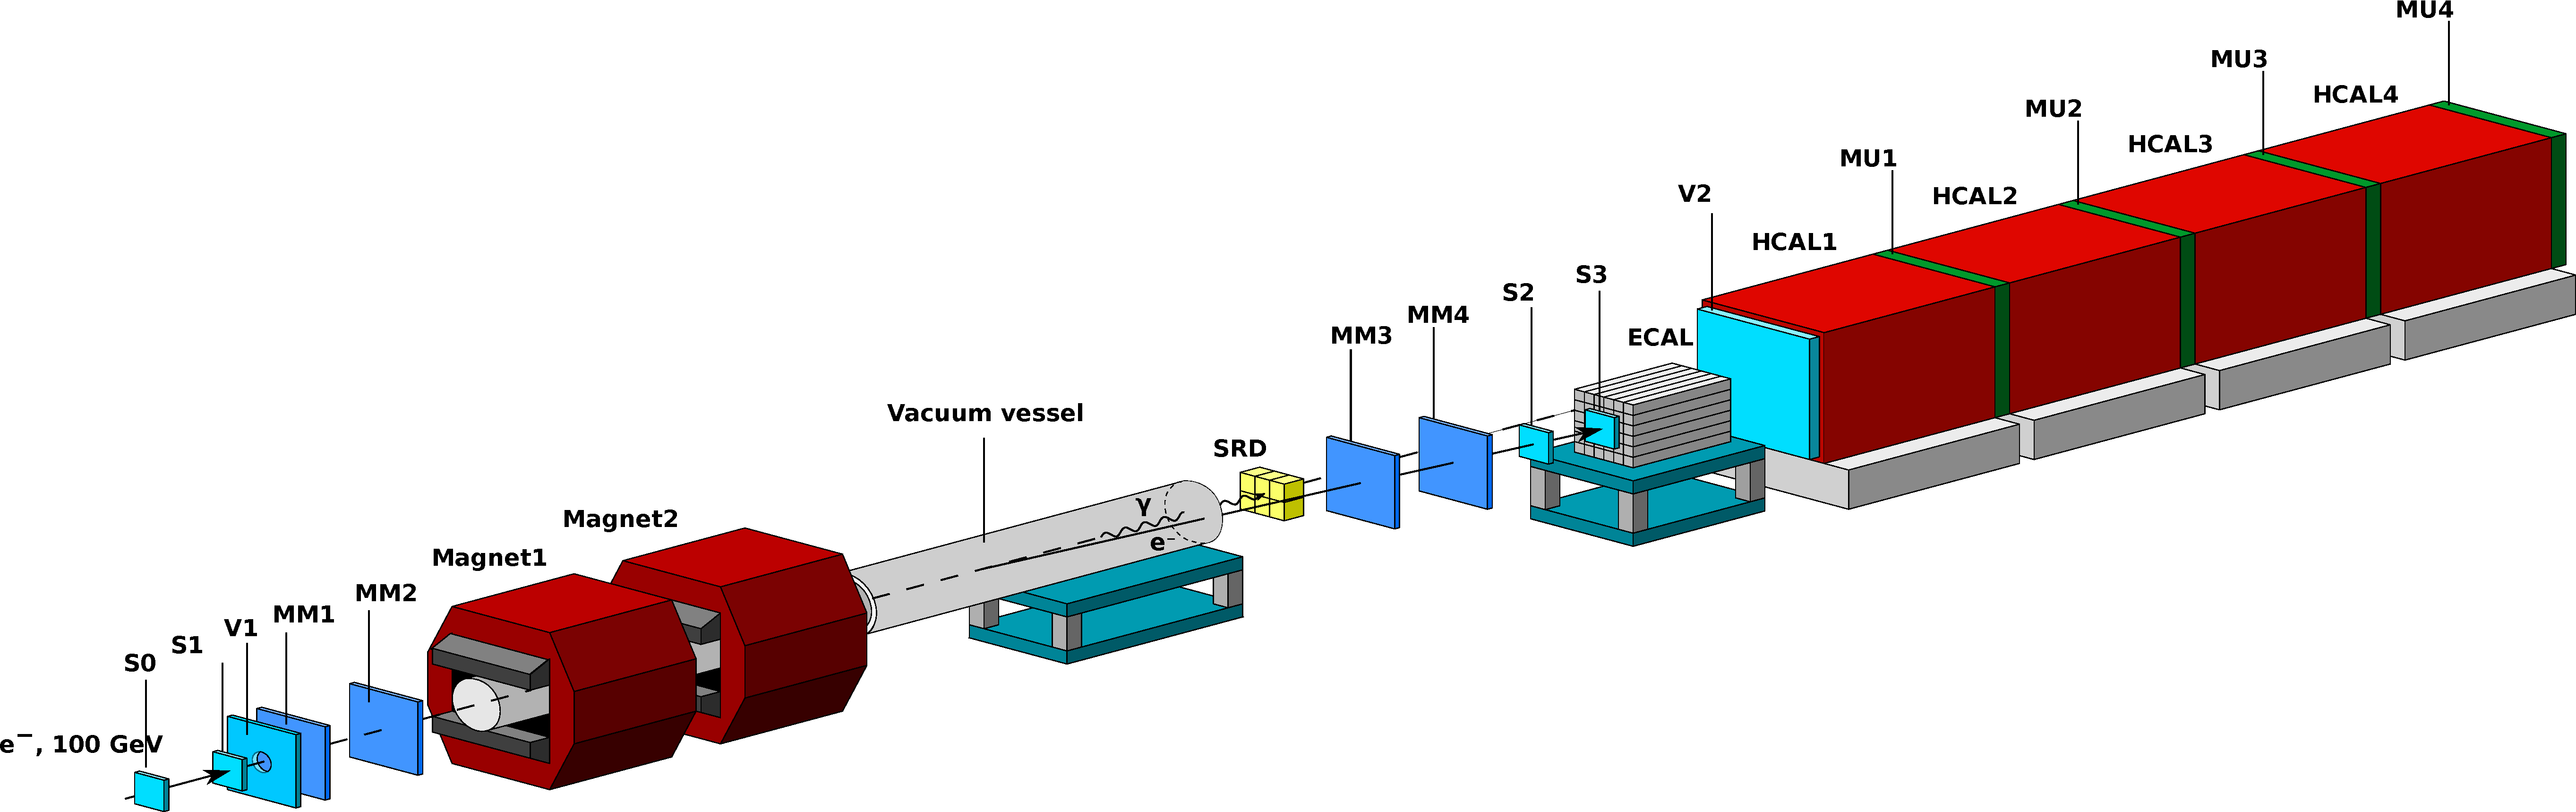
\includegraphics[width=\textwidth]{\pdirtwo/invisible_mode_setup.pdf}
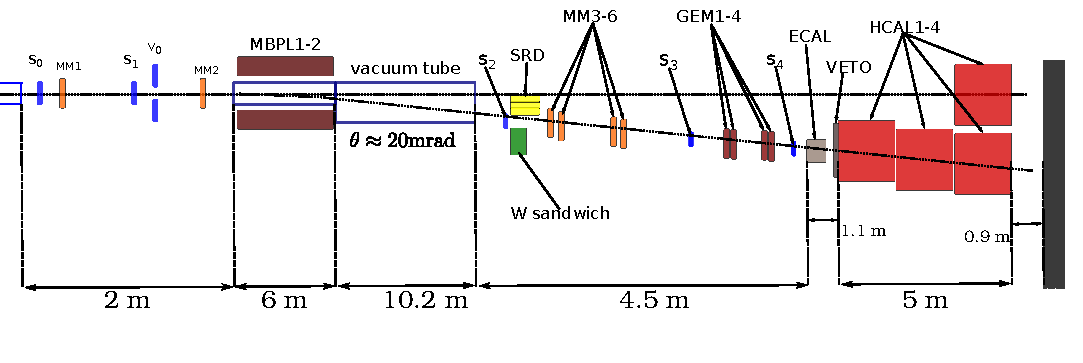
\includegraphics[width=\textwidth]{\pdirtwo/setup-invis-2018.pdf}
\caption[Invisible mode setup 2018]{Top: 3D sketch where the main detectors are shown. Bottom: Top view of the invisible mode setup used in 2018.}
\label{fig:setup-invis-2018}
\end{figure}

\subsection{The visible mode setup}
\label{ch2:sec:vismode}

The invisible mode setup is slightly modified to accommodate a long decay volume where the $\ee$ pair from the $\DM$ decay would be measured by a scintillator counter and four GEM stations (Fig.\ref{fig:setup-vis-2018}). The energy of the beam is increased to 150 GeV\footnote{The first run in 2017 was performed at 100 $\gev$.}. The reason for this is to boost the $\DM$ decays outside the dump. As a consequence, the total displacement of the primary beam caused by deflection in the magnetic field is roughly $\sim$\SI{10}{\milli\meter} smaller. Since the space between the original and the bent beam axis is reduced, only two modules of the SRD detector fit in this space, which decreases the suppression of heavy charged particles as will be detailed in Sec.\ref{ch3:sec:bkg-srd}. Moreover, the smaller bending has an impact on the momentum reconstruction, less significant for the visible mode than for the invisible one searching for missing energy events. A compact calorimeter made of a Tungsten-scintillator sandwich (WCAL) is located in front of the ECAL and acts as the target in this new setup. This calorimeter has a total of 30$X_0$ in a compact length of $\sim$20 \si{cm}. The $\DM$ is produced via scattering off nuclei in the active dump, followed by its decay $\aee$ after traveling for some distance without interaction. The last layer of the WCAL is read separately (W2). This acts as a veto to reject high energetic particles that leak from the em-shower. A vacuum tube of \SI{3.1}{m} kept at $\sim$10$^{-2}$ \si{mbar} is used to minimize interactions of the $\ee$. A scintillator (S$_4$) is placed immediately after the tube to detect the presence of the $\ee$ pair. A set of four GEM detectors is then placed in the last $\simeq$\SI{2.5}{m} of air before the ECAL. These four trackers can reconstruct the angle and the vertex of the decay to offer an additional characterization of the signal. These tools were not used in the analysis performed in 2018 \cite{Banerjee:2019hmi}, but in this thesis, an analysis based on these trackers information is also described (see Sec.\ref{ch3:sec:vis-mode-tracking}). Finally, the ECAL detects the remaining energy of the $\ee$ pair in the decay volume. If the sum $E_{WCAL}+E_{ECAL}$ is compatible with the initial primary energy E$_0$, we conclude that some energy escaped the WCAL through a new physics process. At the end of the setup, a high-efficiency VETO and the HCAL are still present to guarantee complete hermeticity. One could question the usefulness of these detectors here, indeed if we can guarantee that only 150 GeV $e^-$ are in the system, the simple requirement of energy conservation should be enough to reject all backgrounds coming from impurities in the beam. However, the limited energy resolution of the two calorimeters can produce a wrong measurement mimicking energy conservation. The HCAL also serves to reject pileup events which can produce the same effect. In addition, it is used to properly estimate the hadron contamination of the beam and to select rare events containing the interaction $\emu$ where two muons are produced in the dump inside the em-shower. This type of event is crucial for our analysis to properly account for the experiment systematics, both in invisible and visible mode, which makes the HCAL and VETO necessary in both setups.

\begin{figure}[tb]
  \centering
  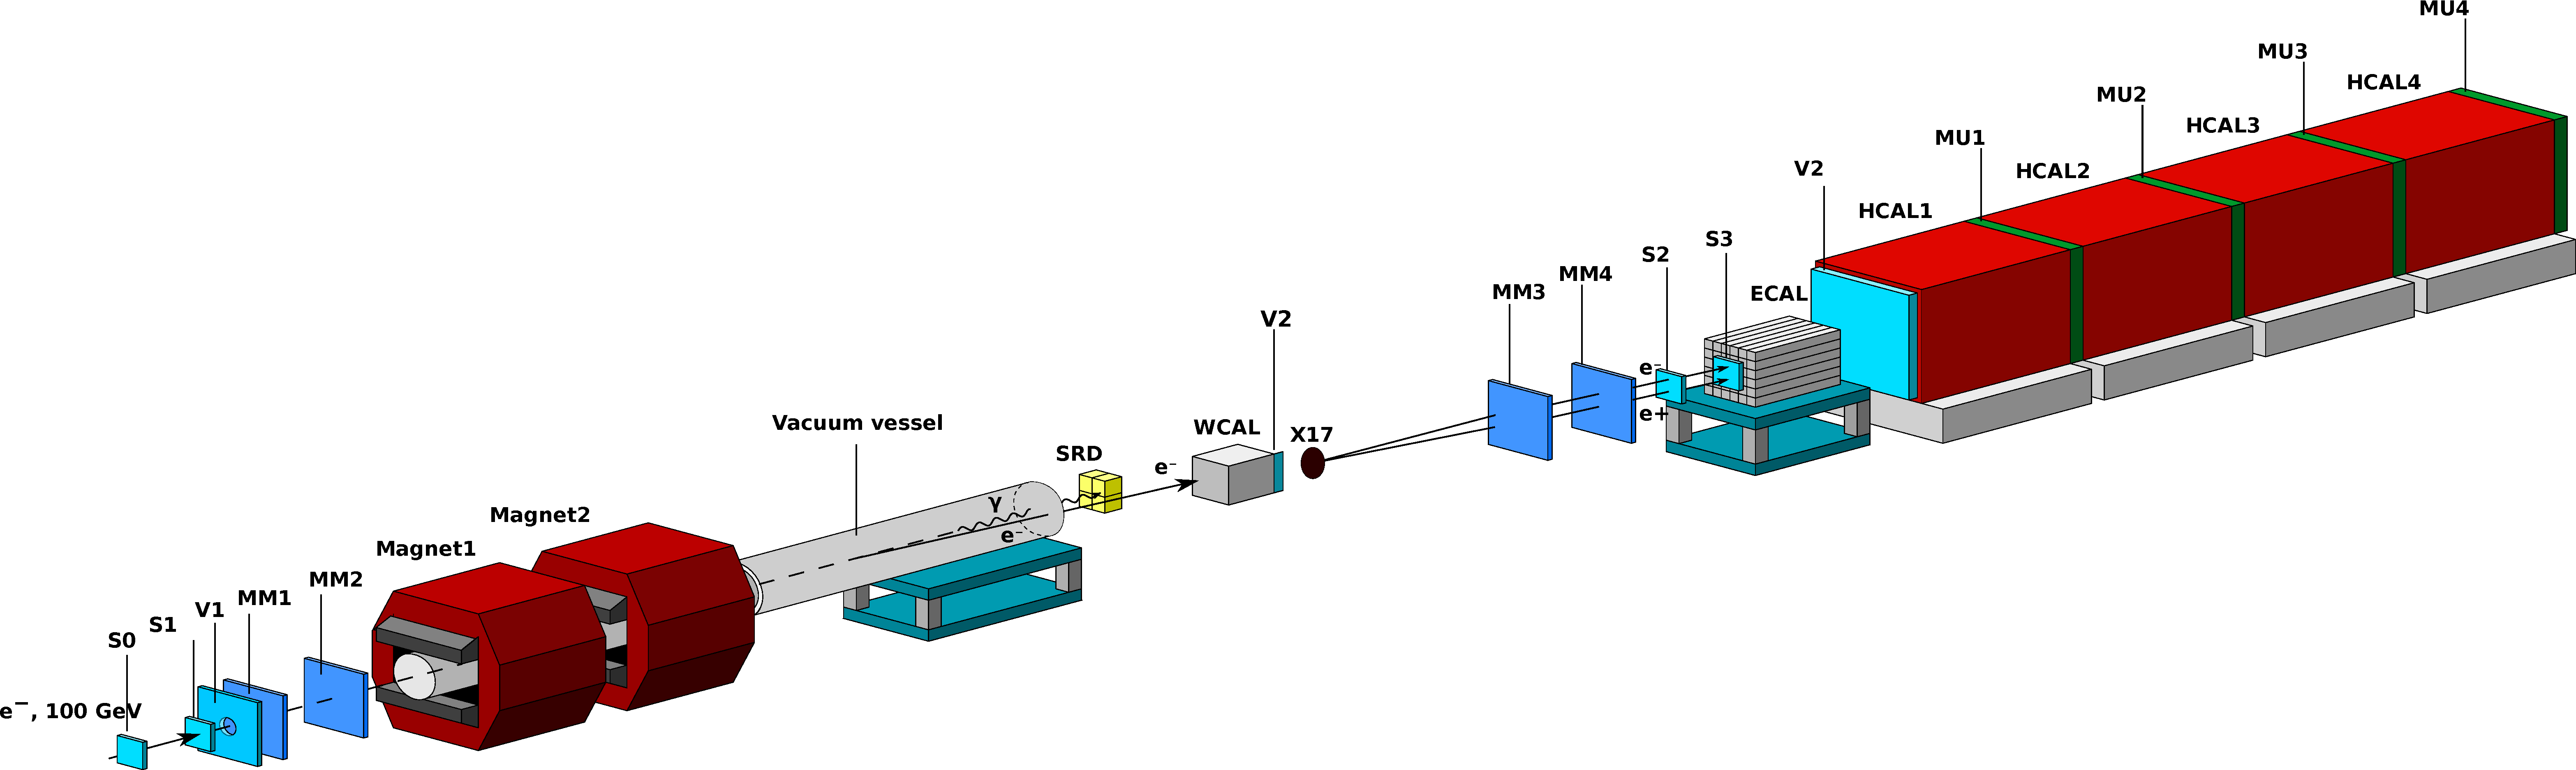
\includegraphics[width=\textwidth]{\pdirtwo/visible_mode_setup.pdf}  
  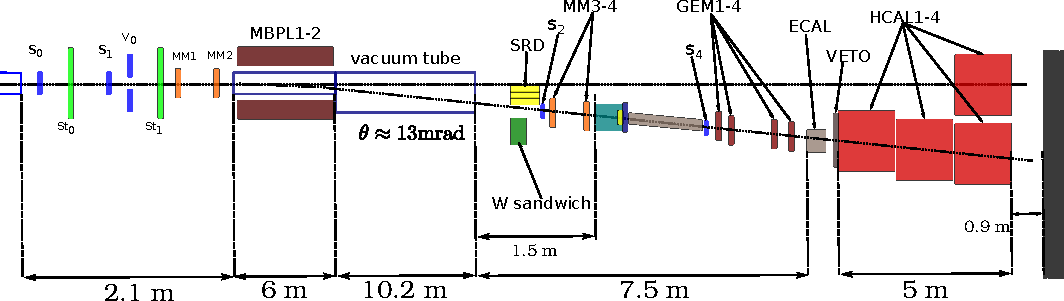
\includegraphics[width=1.\textwidth]{\pdirtwo/NA64_setup_2018_visible.pdf}
  \caption[NA64 visible mode setup 2018]{Top: Visible mode setup sketched in 3D. A decay of the $\DMX$ after the dump is depicted. Main detectors are shown. Bottom: Top view of the visible mode setup used in 2018.}
  \label{fig:setup-vis-2018}
\end{figure}

\section{Detectors}
\label{ch2:sec:detectors}

In this section, a technical overview of each setup component is described in more detail. Additional information about them can be found in \cite{ABBON201569}. A summary with all technical details is also provided in Table \ref{tab:detector-tables}.

\subsection{The Trigger system}
\label{ch2:sec:detectors-trigger}

The trigger system is based on the coincidence and anti-coincidence of different scintillator counters placed along the beam directions combined with the requirement of specific energy in the primary active dump (the ECAL in the invisible mode and the WCAL in the visible mode).

Five plastic scintillators (S$_{0-4}$) and one Veto (V) counter are used for this purpose. They have a variable diameter ranging from 32 to 42 \si{mm} and a thickness of 3-5 \si{mm}. The sandwich S$_0$-V-S$_1$ in front of the beam inlet characterizes the initial particle direction. To pass the first level of the trigger, a particle needs to leave a signal of at least 0.8 $\emip$\footnote{Most Probable Value (MPV) of the energy deposited by a minimum ionizing particle MIP inside the active volume.} in S$_{0-1}$ and no signal in V. This is expressed by the condition:

\begin{equation}
\label{eq:trigger-upstream}
Tr_{\rm{U}} = S_0 \cdot \bar{V} \cdot S_1
\end{equation}

The signal is also required to be in time coincidence ($\simeq$3 \si{ns}) to suppress the pileup. In the invisible mode, three additional scintillator counters are placed (S$_{2-4}$) downstream and a signal in time coincidence in the three detectors is required for the second level of the trigger. For the visible mode search, only (S$_2$) is used for the downstream trigger, S$_3$ is removed and S$_4$ is placed after the decay volume without being a direct part of the trigger. This means:

\begin{equation}
\label{eq:trigger-downstream}
\begin{split}      
& Tr^{\rm{invis}}_{\rm{D}} = S_2 \cdot S_3 \cdot S_4 \\
& Tr^{\rm{vis}}_{\rm{D}} = S_2 \\
& Tr^{\rm{invis/vis}}_{\rm{U}+\rm{D}} = Tr_{\rm{U}} \cdot Tr^{\rm{invis/vis}}_{\rm{D}}
\end{split}
\end{equation}

The scintillator counters downstream are small enough to already limit significantly the range of momenta accepted in the trigger of the experiment ($\gtrsim$ 80 $\gev$). However, primaries with a large initial angle can still be within the acceptance of the setup, hence the necessity of a tracking system. As a final tool for the beam definition, the W counter (located close to the SRD in Fig.\ref{fig:setup-invis-2018}-\ref{fig:setup-vis-2018}) is used as a veto to reject events with large upstream Bremsstrahlung. The exact energy threshold is run-dependent, but it is always in the range of 3-6 $\gev$. We define the beam-trigger as the sum of all these components in the two different setups:

\begin{equation}
\label{eq:trigger-beam}
Tr_{\rm{beam}} = Tr_{\rm{U}+\rm{D}} \cdot \bar{W}
\end{equation}

As the DAQ can collect data at a rate of $\simeq$10 \si{kHz}, an additional condition to avoid the saturation of the system is needed. Therefore, the condition that the incoming electron deposited less than 85 GeV in the ECAL (invisible mode) or WCAL (visible mode) is added to the trigger. This allows to reject SM events and select possible candidate missing energy events. Additionally, since both WCAL and ECAL are segmented longitudinally, one can use the pre-shower information to suppress the hadron background at trigger level. We call this "physical trigger", which takes the form:

\begin{equation}
\label{eq:trigger-phys}
\begin{split}
& Tr^{\rm{invis}}_{\rm{phys}} = ECAL^{\rm{presh}}(> \SI{300}{\mega\electronvolt}) \cdot ECAL(<\SI{85}{\giga\electronvolt})\\
& Tr^{\rm{vis}}_{\rm{phys}} = WCAL^{\rm{presh}}(>\SI{500}{\mega\electronvolt}) \cdot WCAL(<\SI{110}{\giga\electronvolt})
\end{split}
\end{equation}

The final trigger during data taking will be a combination of both the primary trigger and the physical trigger:

\begin{equation}
\label{eq:trigger-total}
\begin{split}
& Tr^{\rm{invis}}_{\rm{total}} = S_0 \cdot \bar{V} \cdot S_1 \cdot S_2 \cdot S_3 \cdot S_4 \cdot \bar{W} \cdot ECAL^{\rm{presh}}(> \SI{300}{\mega\electronvolt}) \cdot ECAL(<\SI{85}{\giga\electronvolt})\\
& Tr^{\rm{vis}}_{\rm{total}} = S_0 \cdot \bar{V} \cdot S_1 \cdot S_2\cdot \bar{W} \cdot WCAL^{\rm{presh}}(>\SI{500}{\mega\electronvolt}) \cdot WCAL(<\SI{110}{\giga\electronvolt})
\end{split}
\end{equation}

Based on the trigger used and the beam settings we can define three different run types:

\begin{itemize}
\item \textbf{Hadron calibration run:} The $\pi^-$ is the primary particle and the trigger is defined as $Tr_{\rm{beam}}$. These runs are used to measure the hadron interactions in the setup and to study the background suppression in NA64. Their intensity is suppressed compared to the electron beam ($\approx 10^{3}$ $\pi^-$\si{\per\second}).
\item \textbf{Electron calibration run:} The $e^-$ is the primary particle and the trigger is defined as $Tr_{\rm{beam}}$. These runs are used to characterize the electron interaction in the setup and its identification efficiency without the physical trigger condition. 

\item \textbf{Physical run:} Where $e^-$ is the primary particle and the trigger is defined as $Tr_{\rm{total}}$. These runs are used to collect the data for the analysis. 
\end{itemize}

Although the Physical runs use an electron beam, the physical trigger naturally selects events with hadrons as a primary particle. The vast majority of $e^-$ will deposit all their energy inside the target-dump and are thus rejected by the physical trigger. This means that the sample of events recorded will have a large percentage of hadrons that will be rejected by the selection criteria. To properly account for the cuts efficiency, electron and hadron calibration runs are used, since the impurity of the sample is known and easy to remove.

\subsection{The Electromagnetic Calorimeter (ECAL)}
\label{ch2:sec:detectors-ecal}

The electromagnetic calorimeter shown in Fig.\ref{fig:ecal-sketch} is a shashlik type detector designed for energy and shower profile measurements and $e/\pi$ separation. Its design consists in a 6$\times$6 matrix of single modules with dimension 38.2$\times$38.2$\times$471 $\mmc$. Each cell is made of 150 layers, with a structure of 1.5 $\mmi$ as converter layer, 0.14 $\mmi$ paper separator, and a 1.5 $\mmi$ scintillator as the active material. This amounts to a total thickness of 40$X_0$ radiation length. Each cell is further divided into two different longitudinal segments. The first one is called pre-shower and consists of 16 layers ($\sim$4.27$X_0$) and provides information on the initial shower shape. Since $e^-$ and $\gamma$ trigger an em-shower as soon as they enter the target\footnote{with the $\gamma$ being a bit delayed within respect to the electron see \cite{Bichsel:2002cf}}, this information can be used to discriminate such particles from all the ones with higher penetrating power (mostly $\pi^-$ and $\mu^-$ in the NA64 case). The second longitudinal segment consists of 134 layers ($\sim$35.73$X_0$) and has the purpose of stopping the incoming particle to measure its energy. The light collection of the scintillator part is performed by WaveLength Shifting (WLS) fibers BCF91a \cite{wls-fibers} inserted in a spiral along the cell to avoid any energy leak. The calorimeter is calibrated using a low-intensity electron beam where a mechanical support structure is used to center in turn every single cell with the beam center. The pre-shower and the main calorimeter are then calibrated using a Gaussian fit. The energy fraction between the two longitudinal segments is calculated through a detailed MC simulation. The energy resolution estimated for this detector is of $10\% / \sqrt{E[\gev]}$.

\begin{figure}[bth!]
\centering
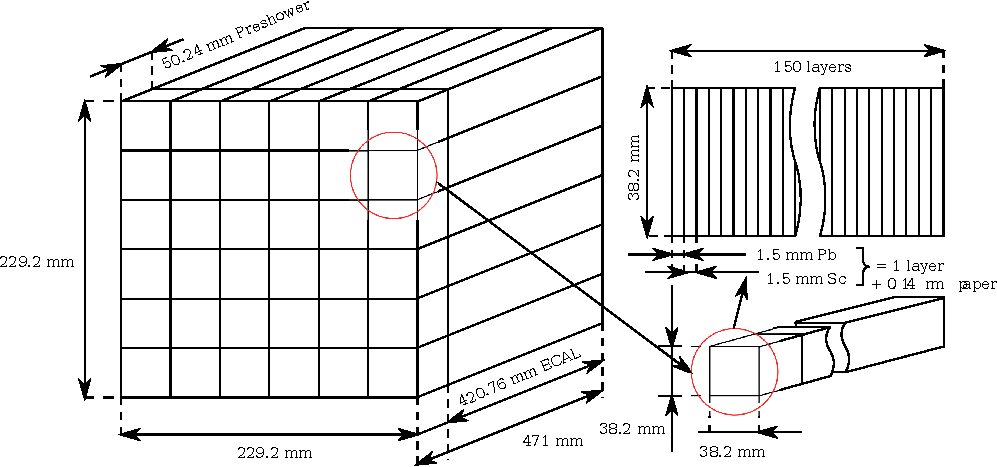
\includegraphics[width=\textwidth]{\pdirtwo/ECAL.pdf}
\caption[ECAL sketch]{Technical sketch of the Shaslik type calorimeter.}
\label{fig:ecal-sketch}
\end{figure}

\subsection{The Tungsten Electromagnetic Calorimeter (WCAL)}

The WCAL is the active target in the visible mode search and it was designed to increase the sensitivity to particles with a short decay length. It is also a shashlik type detector designed to stop high-energy particles in a short length (see Fig.\ref{fig:wcal-sketch}). Its structure consists of a sandwich of Tungsten and scintillator counters for a total of 35 layers. Each layer is made of 3 $\mmi$ Tungsten and 2 $\mmi$ of scintillator material, for a total radiation length of $\sim$30$X_0$. Its dimension is 150$\times$150$\times$200 $\mmc$, including the Aluminum box used to hold the detector together. The total transverse size of the active area is 120$\times$120 $\mms$. The readout is the same used for the ECAL and has a total energy resolution of $20\%/ \sqrt{E[\gev]}$. The WCAL is not segmented transversely but only longitudinally in three different sections. The first one, called pre-shower, is composed of 5 layers to increase the $e/\pi$ separation. The second one is the main calorimeter, made of the remaining 30 layers, used to stop the incoming $e^-$ and measure their energy. The last part is the veto, called W2, made of three scintillator counters stacked in series and read out by a single PMT. It has a total active dimension of 60$\times$120$\times$120 $\mmc$. The purpose of this last detector is to reject charged particles leaking in the decay volume.

\begin{figure}[bth!]
\centering
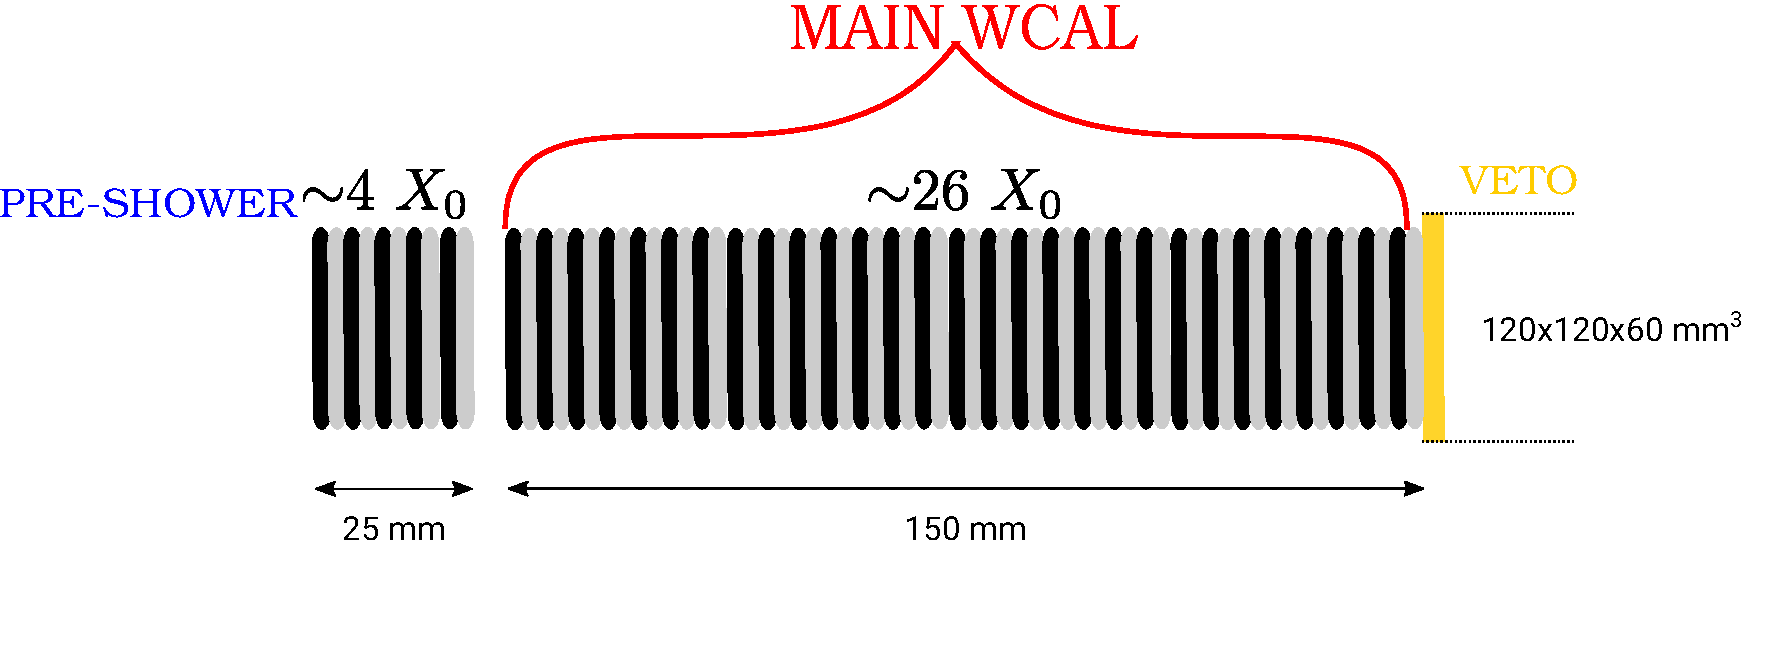
\includegraphics[width=\textwidth]{\pdirtwo/WCAL.pdf}
\caption[WCAL sketch]{Sketch of the WCAL module used in the NA64 experiment.}
\label{fig:wcal-sketch}
\end{figure}


\subsection{The Hadronic Calorimeter (HCAL)}
\label{ch2:sec:detectors-hcal}

The HCAL has the primary purpose to stop and reconstruct the energy of a high penetrating particle. Mostly these particles, $\pi^-$, and $K^-$, are present as impurities in the beam, but also neutrons and protons are produced in inelastic scattering in the ECAL. Although 100 GeV $\mu^-$ will still punch through, the HCAL can measure efficiently the presence of such particles after the ECAL. The $\mu^-$ will leave a distinctive $\emip$ energy deposit inside each module, amounting roughly to $\sim 2.5$ $\gev$. Each module of the HCAL is a 3$\times$3 cell matrix, consisting of alternating layers of 25 $\mmi$ Iron (Fe) and 4 $\mmi$ of scintillating material separated by a 9 $\mmi$ gap of air. Each cell consists of 48 layers for a total thickness of $\simeq 7\lambda_{int}$. The lateral size of each module is 194$\times$192 $\mms$. The light readout is analogous to the one of the ECAL: WLS-fibers embedded in round grooves in the scintillator plates. The fibers from each cell are collected together in a single optical connector at the side of the module which is then read-out by a single photomultiplier. Similar to the ECAL, these modules are calibrated using special runs where 50 $\gev$ $\pi^-$ are shot at different cells. The energy resolution estimated for this detector is $\sim 50\%/\sqrt{E[GeV]}$

\begin{figure}[bth!]
\centering
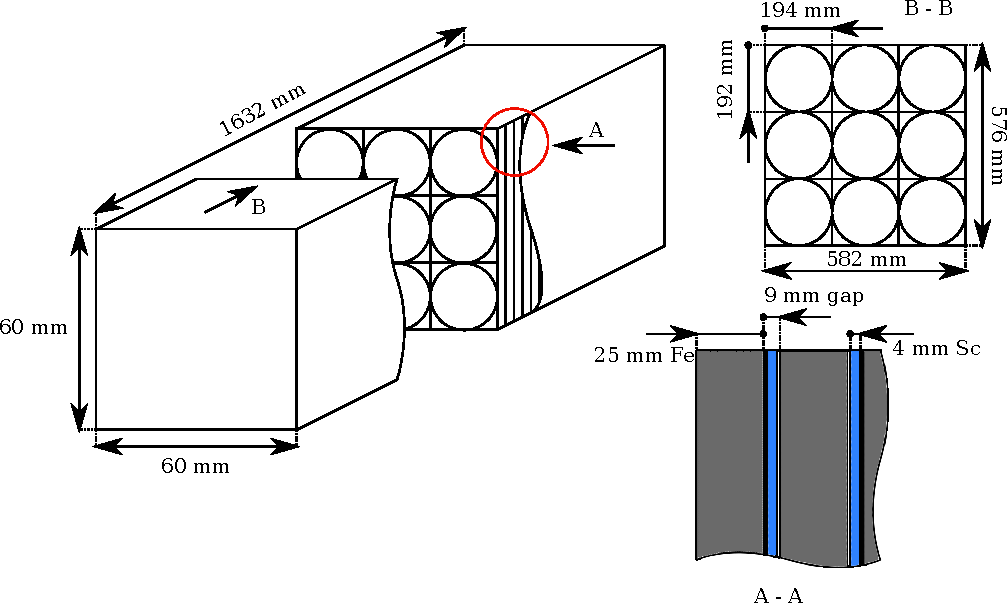
\includegraphics[width=\textwidth]{\pdirtwo/HCAL.pdf}
\caption[HCAL sketch]{Technical sketch of the HCAL module used in the NA64 experiment.}
\label{fig:hcal-sketch}
\end{figure}

\subsection{The Synchrotron radiation detector (SRD)}
\label{ch2:sec:detectors-srd}

The SRD is a calorimeter placed downstream in the arc described by the original beam axis and the bent beam. Its purpose is to measure the energy of the photon emitted during the passage of each electron in the magnetic field. The energy range of such a signal is in the order of a few tens of MeV, two orders of magnitude smaller than the primary beam energy. Heavy charged particle suppression will be described in Sec.\ref{ch3:sec:bkg-srd}.

The first version of the Synchrotron radiation detector used was a set of 8 BGO crystals arranged in a 2$\times$4 matrix parallel to the beam direction. The installation of this detector and the analysis of the data collected was my responsibility. Each crystal has a hexagonal shape with a diameter of 61 $\mmi$ and a length of 200 $\mmi$. The light produced is readout through an EMI PMT 9603 mounted on the bottom of each crystal with optical grease. The BGO crystals are excellent candidates for the SRD, due to their high light-yield and radiation length which coupled to their high Z makes them very good gamma-absorbers \cite{bgo-crystal}. The rejection power experimentally achieved was $10^{-5}$ (see Sec.\ref{ch3:sec:bkg-srd} for details). However, their relatively long decay time of $\sim$300 \si{ns} limits significantly their usability for high-intensity beams.

The BGO detector was essential to validate the method to reject heavy charged particles. Additionally, it demonstrated that the granularity of the detector can be used to improve the hadrons rejection by two orders of magnitude (see Sec.\ref{ch3:sec:bkg-srd}). The BGO detector was substituted with a shashlik type detector in 2017, which uses three adjacent cells of dimension 60$\times$80 $\mmi$. Each cell is made of 100 lead-scintillator layers with dimensions 0.1 $\mmi$ and 1.1 $\mmi$ respectively. The light is read out by an R9420-100-10 Hamamatsu PMT with extended green spectral sensitivity \cite{hamamatsu-R9420-100-10}. The time resolution for the shashlik type SRD is $\sim$5 \si{ns}, which minimizes the pileup from the electrons high-rate provided by the H4 beamline.

\begin{figure}[bth!]
\centering
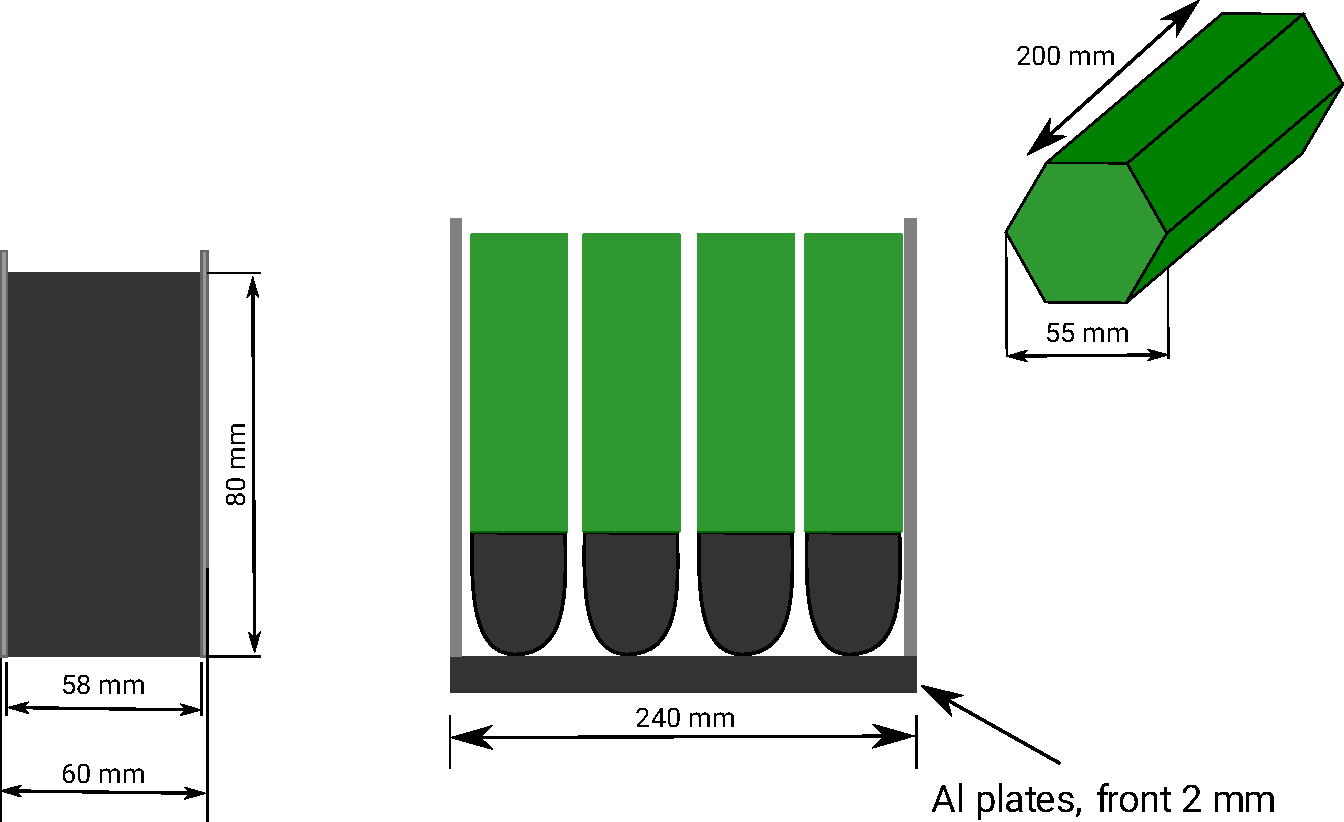
\includegraphics[width=\textwidth]{\pdirtwo/BGO.pdf}
\caption[BGO sketch]{Technical sketch of BGO crystal array.}
\label{fig:bgo-sketch}
\end{figure}

\begin{figure}[bth!]
\centering
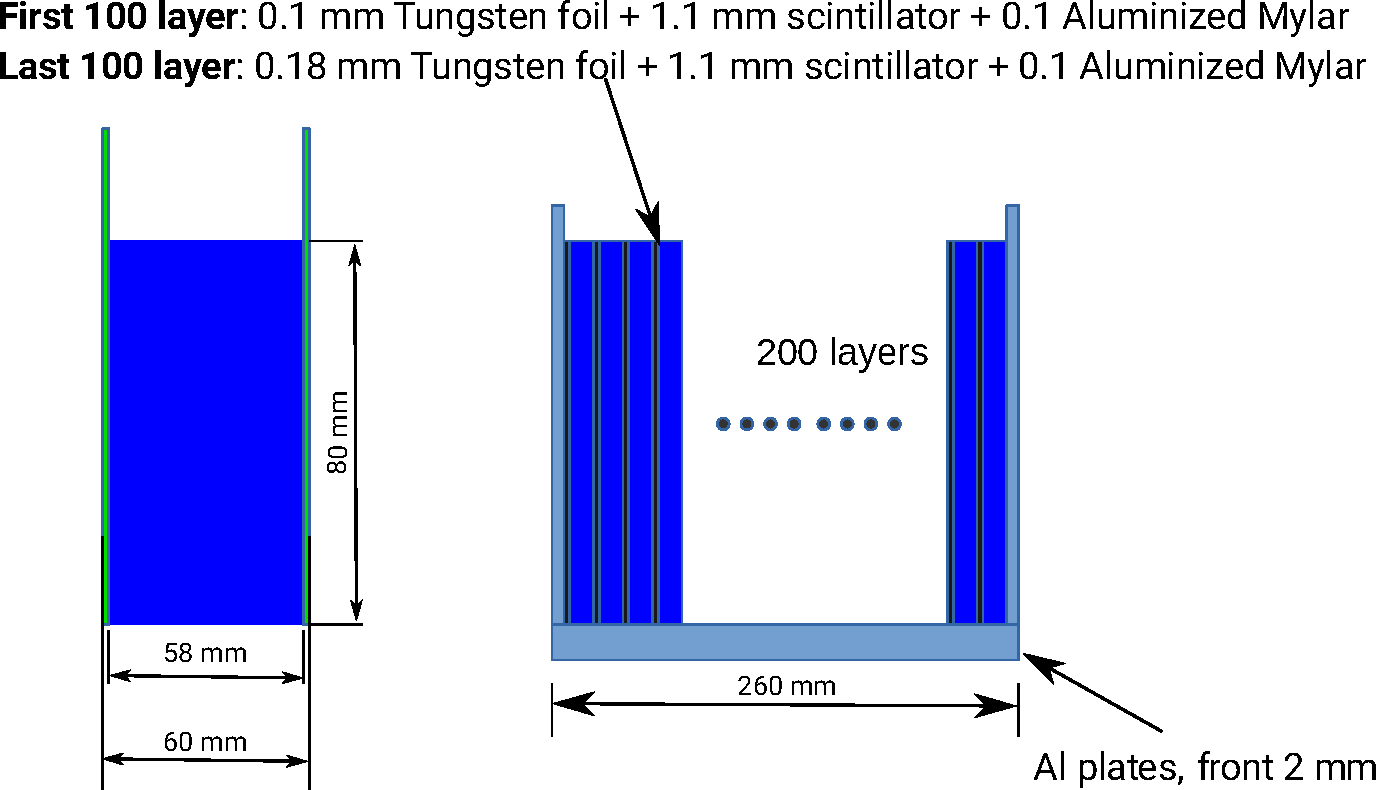
\includegraphics[width=\textwidth]{\pdirtwo/SRD.pdf}
\caption[SRD sketch]{Technical sketch of a single shashlik type module used in the NA64 experiment as SRD.}
\label{fig:srd-sketch}
\end{figure}

\subsection{The Veto system}
\label{ch2:sec:detectors-veto}

The Veto system is the set of scintillator counters measuring charged particles penetrating the main active target.

The most relevant detector of this type is the VETO, a set of three scintillators mounted in series for a total dimension of 550$\times$550$\times$50 $\mmc$. Its MIP inefficiency was estimated to be $\lesssim 10^{-3}$ by using muons from hadron calibration runs.

For the visible mode, it is crucial to maintain the dump as short as possible to increase the probability of the $\aee$ decay to be outside of the dump. For this purpose, the last layers of the WCAL sandwich are decoupled from the main readout and used as a veto (called W2). For testing purposes, a second thicker counter (called V2) is still placed at a distance of $\sim3$ \si{cm} from W2 to cross-check its efficiency.

In general, a signal event in both visible and invisible mode is characterized by the absence of energy in the veto counter placed behind the target dump. In practice, events with an energy deposit $<$0.8 $\emip$ are accepted, taking into account both pedestal and energy resolution of these detectors.

\subsection{The Tracking system}
\label{ch2:sec:detectors-tracking}

The tracking system is a group of detectors that allows the momentum reconstruction and track propagation in the NA64 setup. Four types of detectors are used to reconstruct hits position: Micromegas (MM), Gas Electron Multiplier (GEM), and Straw chambers (St). To this date, only MM trackers are used as a direct part of the tracking system. In this thesis, however, a new analysis of the visible mode data is performed by exploiting the GEM trackers information to reconstruct tracks in the decay volume.

The exact working principle of each of these detectors is beyond the scope of this thesis. This section will mainly cover Micromegas detectors, which were also my main responsibility during data taking. More information on the NA64 Straw chamber can be found in \cite{pdegen-thesis}.

\subsubsection{Micromegas}

Micromegas trackers are a set of eight Multiplexed XY Resistive Micromegas detectors (MM$_{1-8}$) used to reconstruct the 2D hit position of the incoming particles. In this section, we will review its working principle and characteristics \footnote{The first modules design and original testing were the topics of a previous thesis \cite{dbanerjee-thesis}}.
As shown in Fig.\ref{fig:mm-sketch}, the primary particle enters the gas box where it produces secondary electrons through ionization. The gas used is a mixture of Argon (93\%) and CO2(7\%). While Argon is used to produce the secondaries, the CO2 acts as a quencher to absorb UV-light emitted to avoid an excessive ionization that would both decrease the hit resolution and saturate the detector. The secondary electrons are then guided by the drift field in the amplification gap. This is separated from the drift gap with a mesh formed by 400 wires with an aperture size of $\sim$45 $\mum$, $\sim$18 $\mum$ wire diameter, and $\sim$ 29 $\mum$ thickness. As pointed out in \cite{Bortfeldt:2014vvt}, an electric field of \SI{0.6}{\kilo\volt\per\centi\metre} in the drift gap is a good compromise to maximize the mesh transparency and ensure an effective propagation of the electrons in the amplification gap. The electrons reaching the amplification gap experience a high electric field of $\sim$\SI{50}{\kilo\volt\per\centi\metre} which triggers a secondary avalanche multiplying the electrical charge, finally collected by the strips on the PCB\footnote{Printed Circuit Board}.
The thin amplification region makes MM particularly vulnerable to sparks, which happen when the total number of electrons in the avalanche reaches the value of a few $\sim 10^7$, called Raether limit \cite{BAY2002162,BRESSAN1999321,Raether:102989}. In addition to possible damage to the detector and the readout electronics, a spark can also lead to dead time, significantly reducing the efficiency of the MM. The introduction of resistive strips, which add a continuous RC circuit on the top of the readout strip plane, leads to the spreading of charge which avoids spark development and voltage drop. These strips are grounded and separated from the readout strips via a thin insulating layer. The charge is therefore not directly collected by the copper strips. Instead, an electrical signal is generated via capacitive coupling between the resistive and readout strips.

\begin{figure}[bth!]
  \centering
  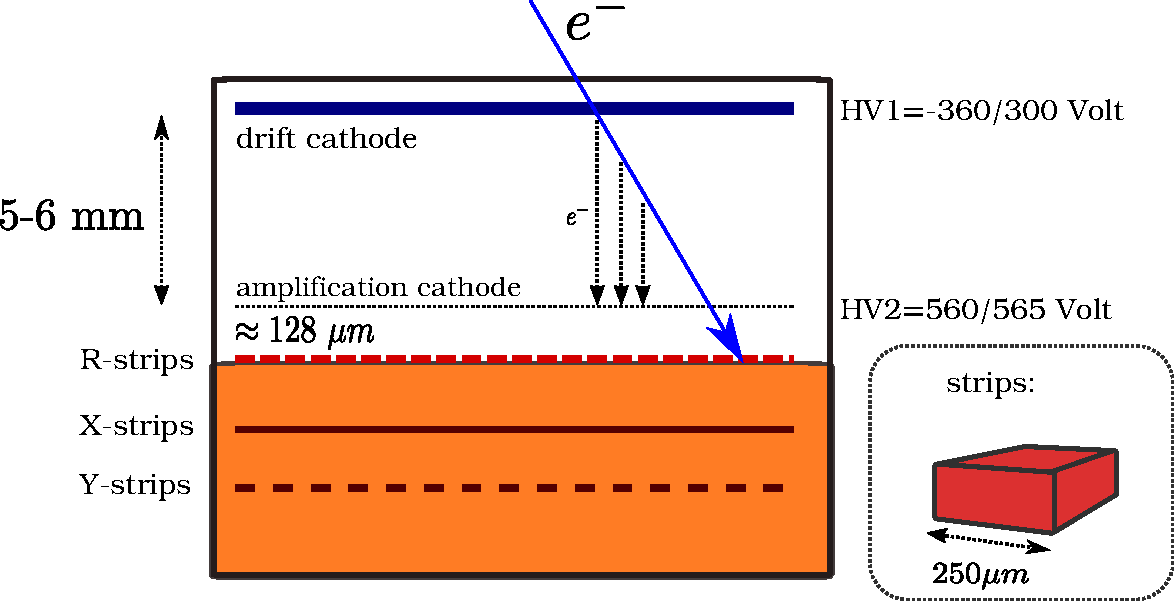
\includegraphics[width=\textwidth]{\pdirtwo/mm-principle.pdf}
\caption[Micromegas sketch]{Working principle and sketch of the NA64 Micromegas detector.}
\label{fig:mm-sketch}
\end{figure}

In the NA64 case, a negative voltage of 300-360 \si{\volt} (depending on the variable drift height) is applied to the drift plate. The mesh is connected to the ground while the resistive strips are kept at a positive voltage ranging from 560 and 565 \si{\volt}. The resistive strips (R-strips) have a resistance of 1 \si{\mega\ohm} and are placed parallel to the X-strips. The Y-strips are placed after the R-strips and perpendicular to them. All set of strips have a pitch of 250 $\mum$, with a width of 200 $\mum$ for the R/X-strips and 50 $\mum$ for the Y-strips.

Another important feature of this detector is the genetic multiplexing of the strips, which are grouped in sets of five connected to a single channel. This scheme reduces the total number of channels needed for a complete readout of a module: the 640 strips of each Micromegas (320 strips per plane) can be read by a single APV25 readout chip (see Sec.\ref{ch2:sec:daq}). The disadvantage of this scheme is a possible redundancy of the hit position, which becomes more relevant as the occupancy of the event increases. To suppress this effect, the strips are mapped to maximize the separation between strips connected to the same channel. This technique was originally proposed in \cite{Procureur:2013yea}, and consists of distinguishing the original physical cluster from the one created as an artifact by the multiplexing mapping by selecting as candidates only clusters where multiple neighboring strips show a signal over the threshold. An example of the output in a plane with a multiplexing factor 5 generated by a single electron passing through is illustrated in Fig.\ref{fig:multiplexing-example}. Producing the optimal mapping for the multiplexing where the redundancy is minimal is not a trivial task. Following \cite{Procureur:2013yea}, one can produce an optimal mapping if the number of channels to map is a prime number. If we consider a detector with $n$ strips to be read by a number of channels $p$, we construct $(p-1)/2$ sub-lists containing the channel numbers $p$ according to the formula:

\begin{equation}
\label{eq:mm-multiplexing-mapping}
1 + [(i \times s) \rm{mod} p]
\end{equation}

where $s$ is the number of the sub-list and $i$ is ranging from 0 to $p-1$. In a more general case, Eq.\ref{eq:mm-multiplexing-mapping} can be used when the number of channels is not a prime number. In the NA64 case, where per plane we have a multiplexing factor of 5 and $n=320$, $p=64$, the sub-lists are constructed using a variation of this equation. Instead of using the number $s$ of the sub-list a set of $(p-1)/2$ numbers, $s_i$ is calculated to minimize the distance between neighboring strips mapped to the same channel $p$. The set $s_i$ is typically computed using numerical methods. The map for both planes of the 8 MM used is shown in Table \ref{tab:mm-map-original}. A new improved map is being prepared for the next generation of the NA64 experiment and will be discussed in chapter \ref{chapter5}.

\begin{figure}[bth!]
  \centering
  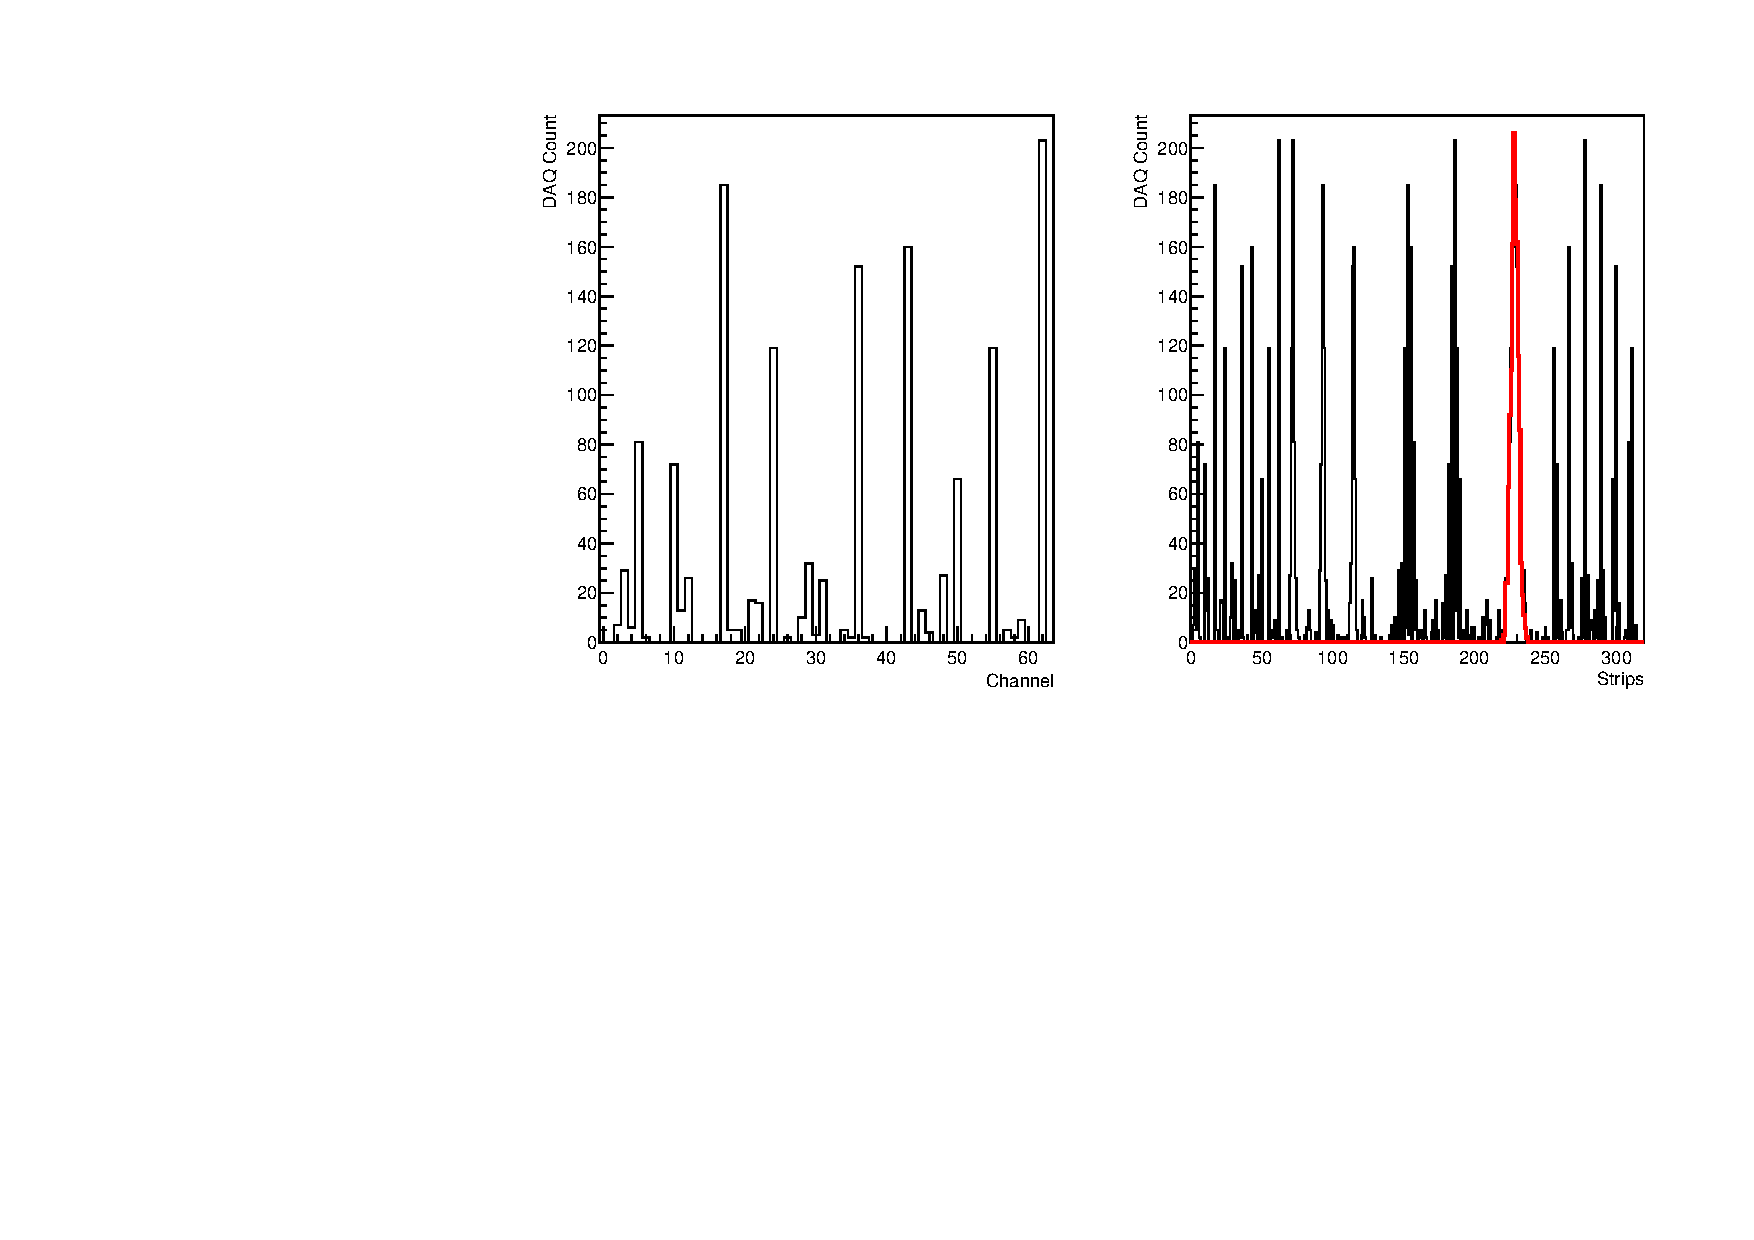
\includegraphics[width=\textwidth]{\pdirtwo/mm_output_example.pdf}
\caption[Example of the readout of a multiplexing detector]{Left: Micromegas plane output after the passage of a MIP. Right: same output transformed in the strips space using the multiplex map. The cluster selected by the reconstruction algorithm is shown in red.}
\label{fig:multiplexing-example}
\end{figure}

In NA64 the multiplexing feature was experimented for the first time in a high-intensity environment. The results show that these trackers are capable to withstand the high flux of particles and allow a precise momentum reconstruction with a precision of $\simeq$1\% at 100 $\gev$ \cite{Banerjee:2017mdu}.

\subsubsection{GEM detectors}
\label{ch2:sec:gem}
The Gas Electron Multiplier (GEM) is a gaseous tracking detector similar to the Micromegas for both active area and performance. The working principle is described in detail in \cite{gem,SAULI20162,ABBON2007455}.

GEM consists of a composite grid of two metal layers separated by a thin insulator (typically Kapton) etched with a regular matrix of open channels. The two metal layers on the opposite side of the grid are kept at a suitable potential difference to create a large field in the hole. Secondary electrons are created by the primary during its passage through the gas and are amplified by the electric field during their drift through the holes. Electrons produced in this multiplication region are then collected by electrodes to measure the impact position of the original particle. To increase the signal, a GEM can stack multiple plates in series to increase the charge multiplication.

In NA64, GEMs were produced using three consecutive foils to amplify the original signal coming from the secondary electrons. This allows the detector to reduce the voltage difference between foils to a minimum to ensure a low amount of discharge. Each foil has an area of 100$\times$100 $\mms$ with a hole pitch of 140 $\mum$. The readout consists of a two-layer strip anode with 256 strips per plane and a pitch of 400 $\mum$. Like the MM, the signal from each strip is processed by 128 channels APV chips, for a total of 4 chips to read both planes.
One of the main differences between the two types of detectors is that GEM trackers are not multiplexed, meaning that every single strip is readout by a single electronic channel. When only one primary particle is present per single event, both MM and GEM performance for momentum reconstruction is similar. For multiple hits in the trackers, a multiplexed detector can create redundancies that limit the efficiency and bias of the reconstructed hit position. For this reason, GEM detectors were placed inside the decay volume during the 2018 visible mode to maximize the efficiency for signal events.

\subsubsection{Straw detectors}

The 2018 invisible mode of NA64 employed three straw trackers in total. Each tracker consisted of two orthogonal planes oriented in the X and Y directions respectively, with each plane consisting of 64 straw tubes arranged in two layers of 32 tubes and glued to each other with a shift of a single tube radius. The tubes had an inner diameter of \SI{6.02}{\milli\metre} and a wall thickness of \SI{62}{\micro\metre}, which was wound of two Kapton tapes. The inner tape was made of Kapton XC160 with a thickness of \SI{40}{\micro\metre} and the outer tape was made of Kapton 100HN with a thickness of \SI{12.5}{\micro\metre} and an aluminized inner surface of \SI{500}{\angstrom}. A gold-plated tungsten wire 30~μm in diameter was used as the anode. The total operating zone covered by each tracker was \num{20 x 20} \si{\square\centi\metre}, in contrast to the \num{8 x 8} \si{\square\centi\metre} of the Micromegas detectors.

Each straw tube was connected to a TDC device, which measured the time interval defined by the timestamps of a start signal and a stop signal. The start signal was given by the signal from the fired straw tube, corresponding to one of the TDC channels 0-63. The stop signal was given by the trigger signal, which was fed into TDC channel 64. The timestamps of both signals were defined by the input amplitude above threshold condition.

A preliminary assessment of the spatial resolution and drift rate of the 6~mm straws carried out in \cite{Volkov:2019qhb} yielded a value of $\simeq$~\SI{250}{\micro\metre} and \SI[separate-uncertainty = true,per-mode=symbol]{14.5(5)}{\nano\second\per\milli\metre} respectively. The drift rate was estimated by reconstructing the position of the incident particle in a MM detector \SI{18}{\metre} upstream of the straw. The expected width of the drift spectrum is roughly 3~mm~$\times$14.5~ns~ = ~43.5~ns, which is consistent with the width of the drift spectrum measured. However, due to non-linearity in the response function, the maximum drift time can reach values slightly higher than that, up to $\sim$60ns.


\subsection{The data Acquisition system (DAQ)}
\label{ch2:sec:daq}

The DAQ used for NA64 is a down-scaled version of the COMPASS DAQ system \cite{Bodlak_2013,COMPASS-daq}. The detector's front-end electronics are connected to the readout modules which have a processing speed up to 160 MB/s. The digital information received by the front-ends is organized into a preliminary event-like structure (see Fig.\ref{fig:daq}). Triggers and control information is passed to these modules via the Trigger Control System (TCS), which work synchronously with the SPS duty cycle and creates the header containing all the event information: spill, event number, and trigger configuration. Two types of readout modules are used in NA64: the CATCH (Compass Accumulate Transfer and Cache Hardware), a general readout module that supports a wide range of front-end electronics, and the GeSiCa (Gem Silicon Control and Acquisition), which is optimized for the readout of the APV25 front-end chip used by MMs and GEMs.

The APV25 is an ASIC that combines analog signals with a digital control \cite{Bodlak_2013} originally developed for the readout of the CMS silicon trackers \cite{article,inproceedings,apv-useguide}. Each of the 128 channels is made of a 60 $\nas$ CR-CR shaping amplifier and a 192 samples deep analog pipeline made of switched-capacitor elements. The amplifier integrates the current pulse from the input and output of a well-defined voltage pulse. The pipeline is then used to store the amplifier output while the chip waits for the external trigger decision. 160 of the 192 memory cells are organized in a ring buffer with a write and trigger pointer. The distance between the two defines the trigger latency which is a configurable parameter. When one of the pipeline columns is flagged for readout, it is copied into one of the remaining 32 memory elements, organized like a FIFO\footnote{\textbf{F}irst \textbf{I}n \textbf{F}irst \textbf{O}ut is a form of data buffer that conserves the order of the incoming data.}. The data are stored here until are sent out by the multiplexer. Then, the data is sent to an ADC\footnote{\textbf{A}nalog to \textbf{D}igital \textbf{C}onverter} modules (able to accommodate 4 APV chip) that digitizes the pulse before sending it to the GeSiCa. The ADC has two possible modes of operation, the latch-all mode, and the sparse mode. When using the latch-all mode, the signal amplitudes of all channels is sampled three times with a clock cycle of 25 $\nas$ and transmitted to the GeSiCa. In this mode the trigger rate cannot be higher than $\sim$1 \si{\kilo\hertz} due to the large amount of data received by the APVs. To reach higher trigger rates, the sparse mode is used instead. When in sparse mode, only channels with amplitudes above a certain threshold are sent to the GeSica by the ADC module. This allows the increase of the manageable trigger rate to $\sim$10 \si{\kilo\hertz}. In NA64, the latch-all mode is used to record the data coming from the APV25 connected to the trackers in absence of the beam. This procedure is repeated every $\sim$10-15 run approximately to record the pedestal of each channel, used to set the threshold (2$\sigma$ for MM and 3$\sigma$ for GEMs) for the sparse mode.

\begin{figure}[tbh!]
\centering
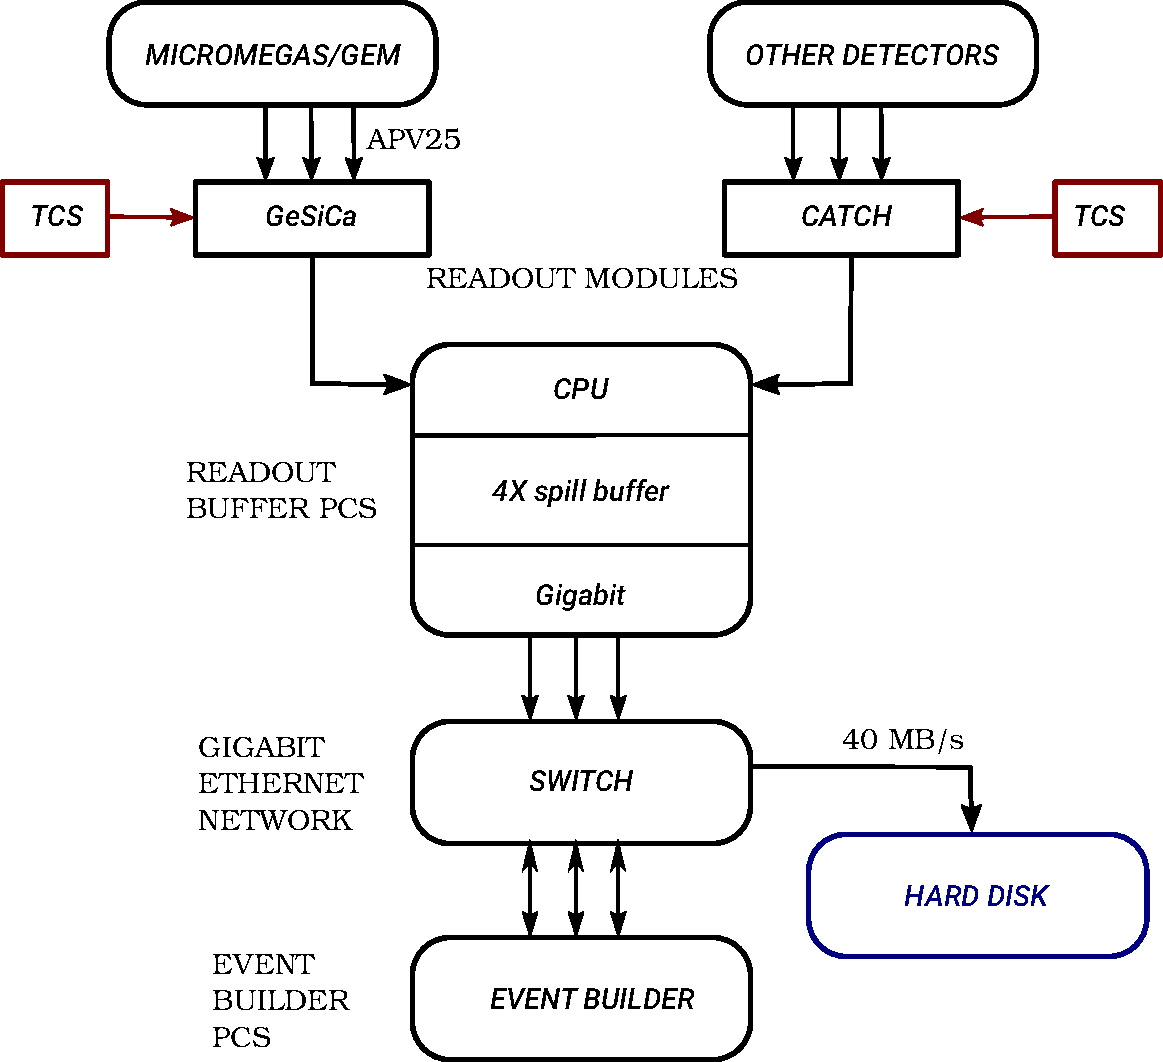
\includegraphics[width=\textwidth]{\pdirtwo/daq.pdf}
\caption{Scheme for the NA64 DAQ}
\label{fig:daq}
\end{figure}

During the calibration procedure, the three samples received by each channel of the APV25 are also used to set the latency of the trigger. This is optimal when it covers the pulse rising edge received by each channel of the APV25. Being a$_0$, a$_1$ and a$_2$ the three sample amplitudes recorded in consecutive order by a single pipeline, the latency is set such that the second sample a$_1$ is larger than the other two. This can be best summarized in the so-called "banana plot" of Fig.\ref{fig:banana-plot}, which is a heat map defined by the frequency of events with certain pulse structure. The sampling of the pulse shape also provides information about the primary electron arrival time. By reconstructing the pulse shape rise time one can improve the estimated time of arrival \footnote{usually 25 $\nas$, limited by the clock frequency of the APV)} down to $\sim$15 $\nas$ \cite{Banerjee:2017mdu}. To achieve this, the pulse is described by the following function:

\begin{equation}
\label{eq:apv-pulse}
r(t) = \frac{r_0}{(1 + \exp{\frac{t-t_0}{\tau}})}
\end{equation}

Where the parameters $r_0$, $t_0$ and $\tau$ are fitted using the same data measured at different values of the latency. The arrival time is then extracted by reversing the expression and solving it as a function of the ratio between pulses:

\begin{equation}
\label{eq:2}
t(r) = t_0 + \tau \times \ln{\frac{r_0}{r} - 1}
\end{equation}

A complete description of the method that takes into account the errors of the ratio and the parameters can be found in \cite{dbanerjee-thesis}.

\begin{figure}[!bth]
  \centering
  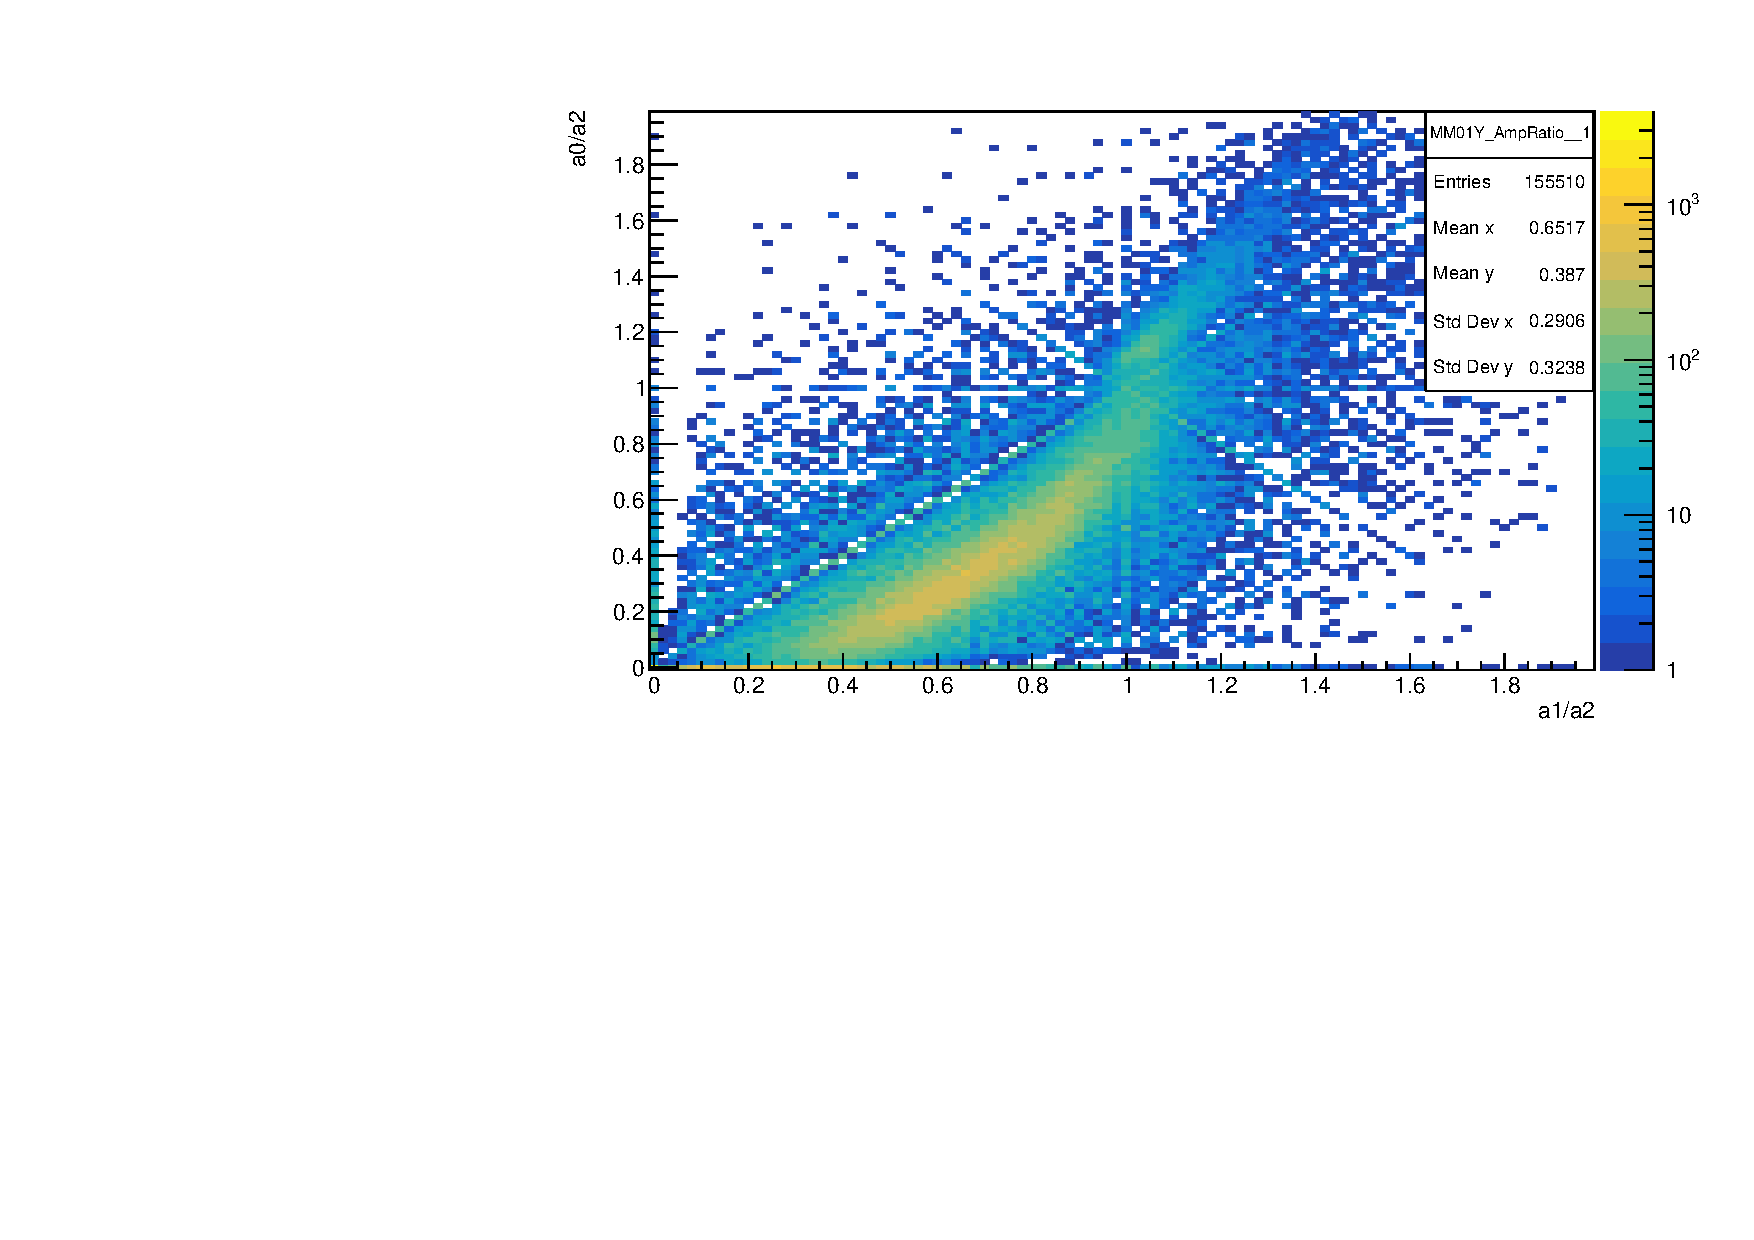
\includegraphics[width=\textwidth]{\pdirtwo/MM1Y_bp.pdf}
\caption[APV25 banana plot]{Ratio between the first two vs the last two amplitudes sampled in an APV25 chip after the proper latency is set for the chip. The typical "banana" shape of this plot shows that the pulse is sampled during its rising edge.}
\label{fig:banana-plot}
\end{figure}

After passing through the ADC, the data is sent to GeSica using a high-speed optical cable. The GeSica can accommodate up to 4 ADC (for a total of 16 APV chips). It has the purpose of multiplexing the incoming data stream, merging the header information from the TCS\footnote{Trigger Control System} with the corresponding data coming from the APV, and putting the event data block into the S-link format. Finally, the information is transferred to a high-performance readout buffer PCs (ROB) via the S-link protocol\footnote{The S-link is a protocol developed at CERN for fast point to point connections, typically between front-end electronics and the readout electronics \cite{s-link}.}. To accommodate many GeSica and CATCH modules, an S-link multiplexer is used to combine the information received by different modules before sending the data to the ROB. The Readout buffer PCs receive the information from the multiplexer and stores them in four different spill buffers\footnote{A spill is a 512 MB SDRAM module that can store the data of at least one spill \cite{COMPASS-daq}}. A Gigabit Ethernet\footnote{Gigabit Ethernet is a standard developed by the Institute of Electrical and Electronics Engineers(IEEE) and Local Area Networks (LANs).} switch connects the ROB with the event builder PC. Here the data of every single event is merged into a single event data block using the event identifier provided by the TCS receiver. After this process, the event is ready to be recorded to the long term storage, in this case a 5 TB SATA Hard Disk with a speed of 40 MB/s. Thanks to this design the DAQ takes advantage of the H4 beam spill of \SI{4.8}{\second}. After the spill buffers are filled, the time before the next spill of $\sim$\SI{20}{\second} is used to build the event and to save all the information processed.

%%% Local Variables:
%%% mode: latex
%%% TeX-master: "../PhDthesis"
%%% End:
